
%%%%%%%%%%%%%%%%%%%%%%%%%%%%%%%%%%%%%%%%%%%%%%%%%%%%%%%%%%%
\section{Experiment}\label{sec:expResults}
%%%%%%%%%%%%%%%%%%%%%%%%%%%%%%%%%%%%%%%%%%%%%%%%%%%%%%%%%%%



%\subsection{Hardware System}


Our experiments are on centimeter-scale hardware systems called \emph{kilobots}.  These allows us to emulate a variety of dynamics, while enabling a high degree of control over robot function, the environment, and data collection. The kilobot, from \cite{Rubenstein2012,rubenstein2014programmable} is a low-cost robot designed for testing collective algorithms with large numbers of robots. It is available as an open source platform or commercially from~\cite{K-Team2015}.  Each robot is approximately 3 cm in diameter, 3 cm tall, and uses two vibration motors to move on a flat surface at speeds up to 1 cm/s.  Each robot has one ambient light sensor that is used to implement \emph{phototaxis},  moving towards a light source. 
In these experiments as shown in Fig.~\ref{fig:setup}, we used $n$=97 kilobots, a glass-covered 1.5 m$\times$1.2 m whiteboard as the workspace, and eight 30W LED floodlights arranged 1.5 m above the plane of the table at the $\{N,NE,E,SE,S,SW,W,NW\}$ vertices of a 6 m square centered on the workspace. The lights were controlled using an Arduino Uno board connected to an 8-relay shield.  Above  the table, an overhead machine vision system tracks the position of the swarm.


\begin{figure}
\begin{center}
	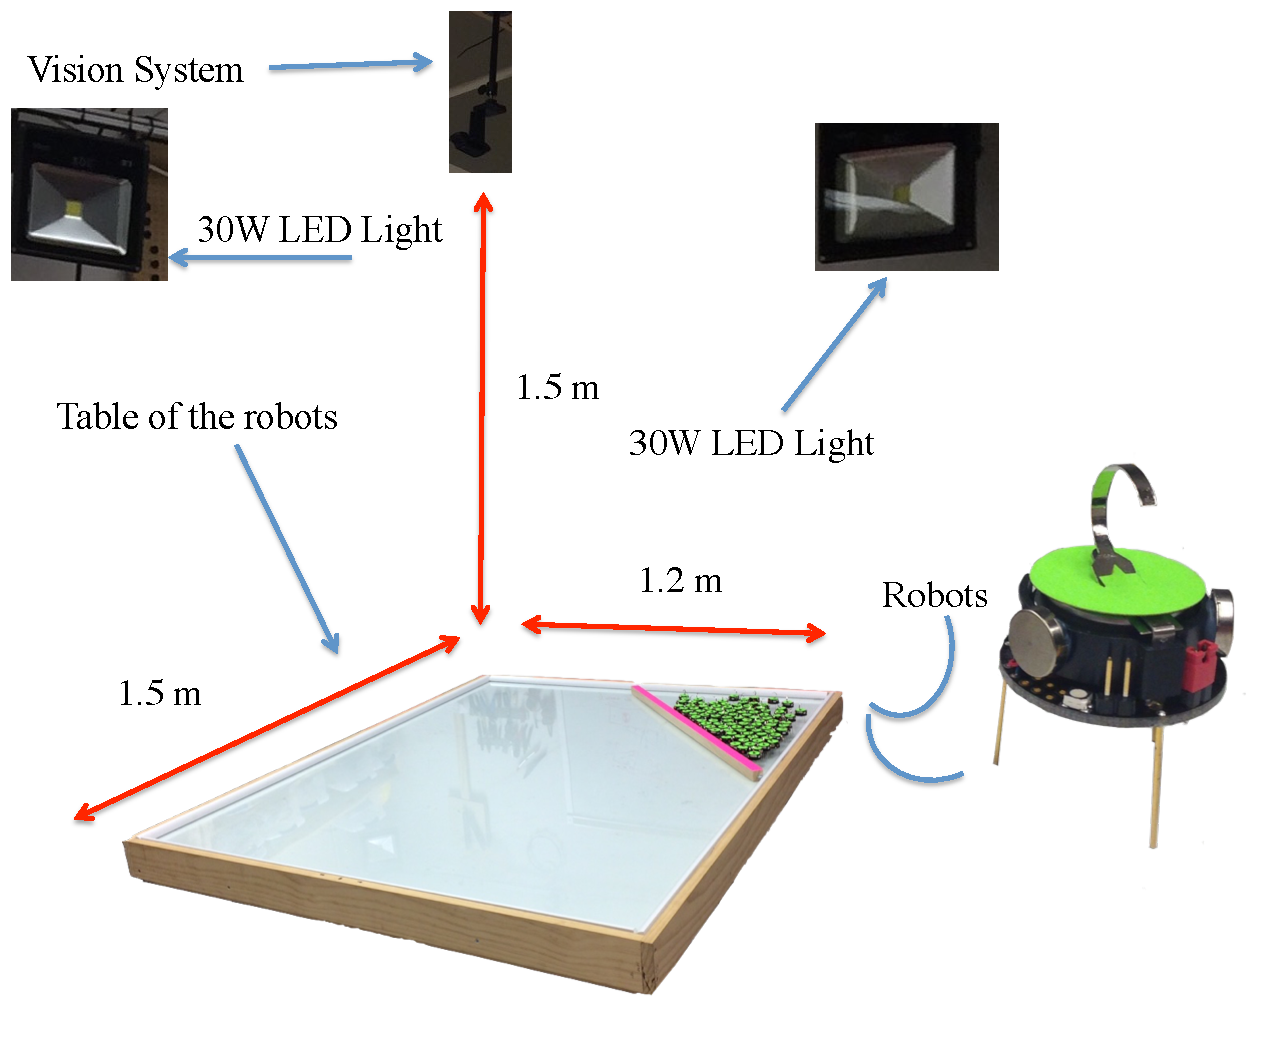
\includegraphics[width=.9\columnwidth]{SetUp.pdf}
\end{center}
\vspace{-1em}
\caption{\label{fig:setup}
Hardware platform:  table with 1.5$\times$1.2 m workspace, surrounded by eight remotely triggered 30W LED floodlights, with an overhead machine vision system.
}
\vspace{-1.5em}
\end{figure}


Fig. \ref{fig:expBig} illustrates the experiment showing pure torque control when we have swarm of robots making force. In this figure the pink object is pivoted to the table, so it can be moved only around its pivot. As we have discussed, the robots will spread highly when we target to push the object from the top. It is because of the features of the swarm. We will have the most torque when the swarm touches the object the most. This is why in Fig. \ref{fig:expBig}, below screenshots have made torque significantly more than the above ones.
\begin{figure*}
\centering
\renewcommand{\figwid}{0.49\columnwidth}
{\begin{overpic}[width =\figwid]{ExpStart.png}\put(6,15){$t$ = 0 s}
\end{overpic}
\begin{overpic}[width =\figwid]{Exp2.png}\put(6,15){$t$ = 30 s}
\end{overpic}
\begin{overpic}[width =\figwid]{Exp2o5.png}\put(6,15){$t$= 120 s}
\end{overpic}
\begin{overpic}[width =\figwid]{Exp3.png}\put(6,15){$t$ = 150 s}
\end{overpic}}\\
\vspace{1em}
{\begin{overpic}[width =\figwid]{ExpStart.png}\put(6,15){$t$ = 0 s}
\end{overpic}
\begin{overpic}[width =\figwid]{Exp4.png}\put(6,15){$t$ = 30 s}
\end{overpic}
\begin{overpic}[width =\figwid]{Exp5.png}\put(6,15){$t$ = 120 s}
\end{overpic}
\begin{overpic}[width =\figwid]{Exp6.png}\put(6,15){$t$ = 150 s}
\end{overpic}}
\vspace{-1em}
\caption{\label{fig:expBig}{Snapshots showing the effect of length of $L$ when we are controlling torque, with 97 robots. The above snapshots illustrates that the swarm will spread out and will not have enough force when $L$ is big. Below show that when the swarm pushes from the middle, mean will not pass the object frequently and it would make enough force. See video attachment. }
%\vspace{-2em}
}
\end{figure*}






